\section{Ausgesuchte Systeme}
\label{sec:Ausgesuchte Systeme}

Zwei der sechs Systeme im \cref{sec:CRS-Git} werden aufgrund deren Eigenschaften, die in der Firma benötigt sind, aufgebaut und getestet. Diese Sind Bitbucket \cref{subsec:Bitbucket} und Gerrit \cref{subsec:Gerrit}.

Folgende Punkte wurden beim Testen betrachtet:

\begin{itemize}
	\item Wie aufwendig der Systems Aufbau ist
	\item Wie kann das Review gestartet und geschlossen werden
	\item Kann eine Pull Request im Vergleich zu den anderen Methoden des Reviews vorteilhaft sein
	\item Erfüllt das System die Kriterien im \cref{sec:kriterien}
\end{itemize}

Nach der Testphase werden die zwei Systeme ausgewertet, miteinander verglichen und deren Vor- und Nachteile vorgestellt.

\section{Testphase}
\label{sec:testphase}

Zum Testen vom Reviews Workflow und von anderen Funktionen der ausgesuchten Systeme \cref{sec:Ausgesuchte Systeme}, wird diese Arbeit, die bereits mit Git versioniert und auf dem Server (Namens odin) der Software-Abteilung gehostet wurde, verwendet, deswegen wird sie in den nächsten Bildern erscheinen.  Die zwei Systeme werden ebenfalls auf odin installiert, wohl wissend, dass auf odin ein Debian läuft. Und Der Reviewer wird der Experte Björn schäpers \cite{Bjoern} sein.

\subsection{Bitbucket}
\label{subsec:Test_Bitbucket}

In den folgenden Unterabschnitten werden die Varianten:
\begin{itemize}
	\item Bitbuckets Webanwendung. Hosten auf Bitbuckets Server
	\item Self-hosten mit Bitbucket-Server
\end{itemize}

vorgestellt und miteinander verglichen.

\subsubsection{Hosten auf dem Server des Anbieters}
\label{subsubsec:Bitbucket-Cloud}

Für den Beginn Verlangt die Webanwendung vom Bitbucket nur eine Anmeldung und schon kann man anfangen, Projekte zu erstellen, in denen die Repositories geklont oder neue erstellt werden können. In dieser Anwendung können auch Funktionen durchgeführt werden, die man mit dem Befehl Line von Git macht. Wie beispielsweise ein neues Branch erstellen, wie in \cref{fig:Bitbucket-Branch-erstellen} zu sehen ist oder ein Repositpry klonen.

\begin{figure}[H]
	\centering
	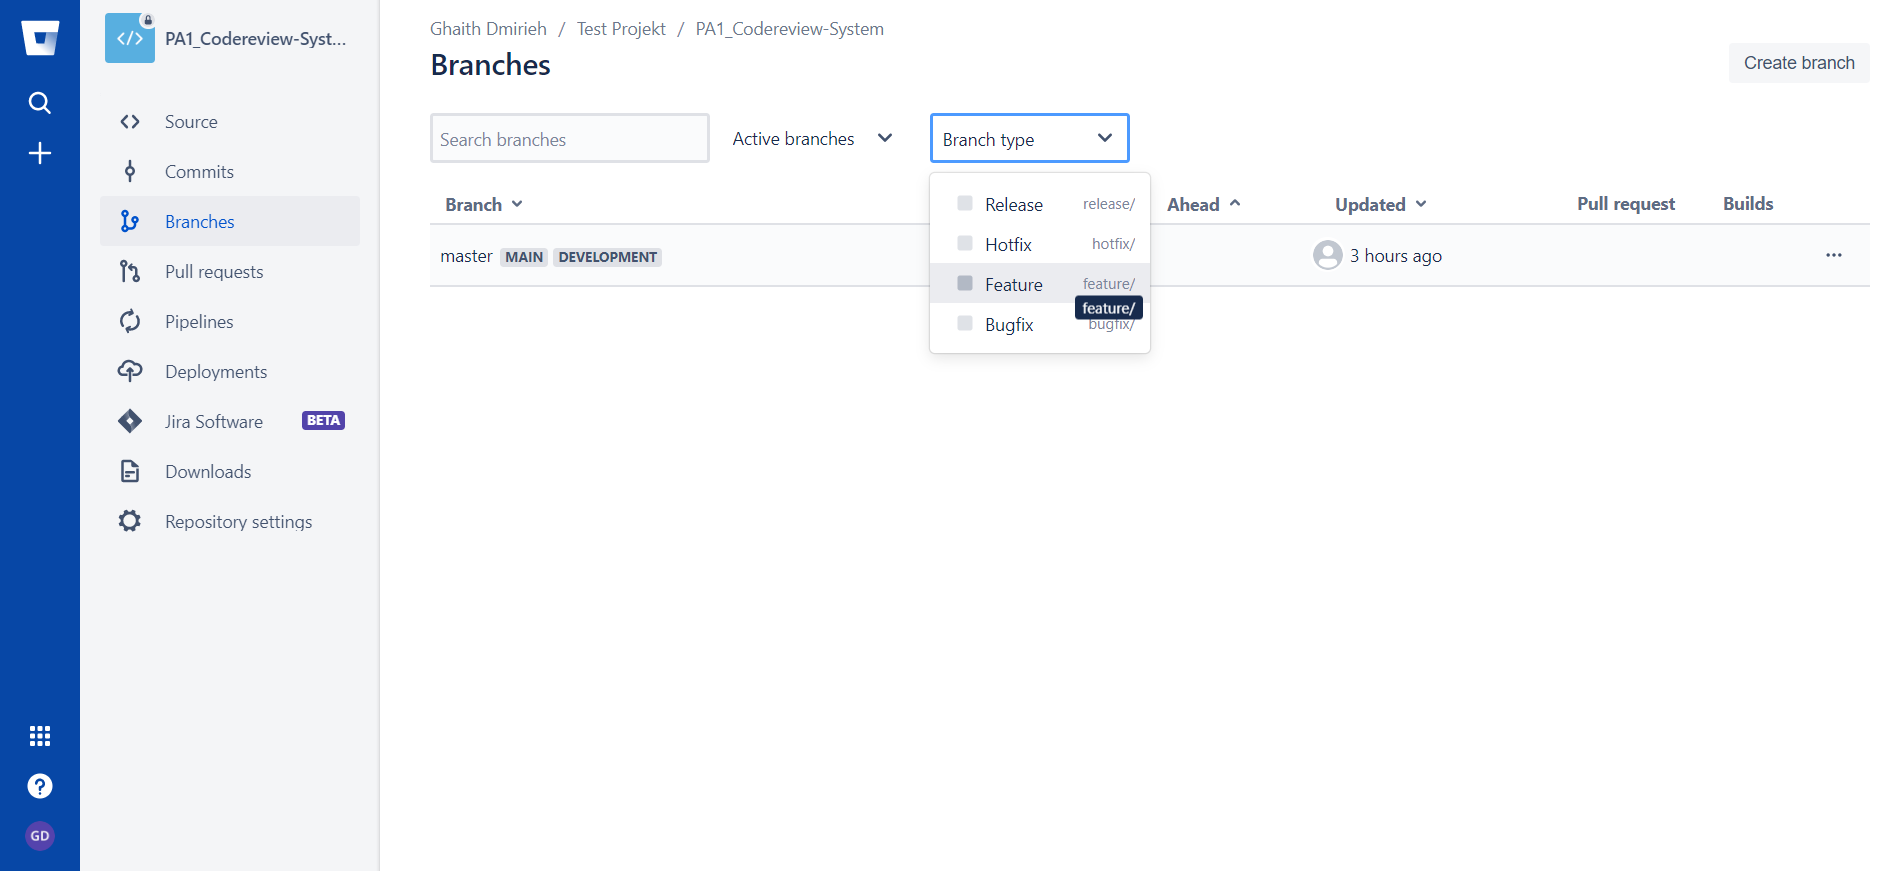
\includegraphics[width=1.0\textwidth]{Bitbucket-Branch-erstellen}
	\caption[Branch auf Bitbuckets Anwendung erstellen]{Ein neues Branch erstellen\\Eigenes Screenshot}
	\label{fig:Bitbucket-Branch-erstellen}
\end{figure}

Die Webanwendung ist imstande, die Änderungsvergleich von jedem commit sowohl inline als auch side-by-side anzuzeigen. Ein Beispiel dafür ist die \cref{fig:Diffs_side-by-side}.

\begin{figure}[H]
	\centering
	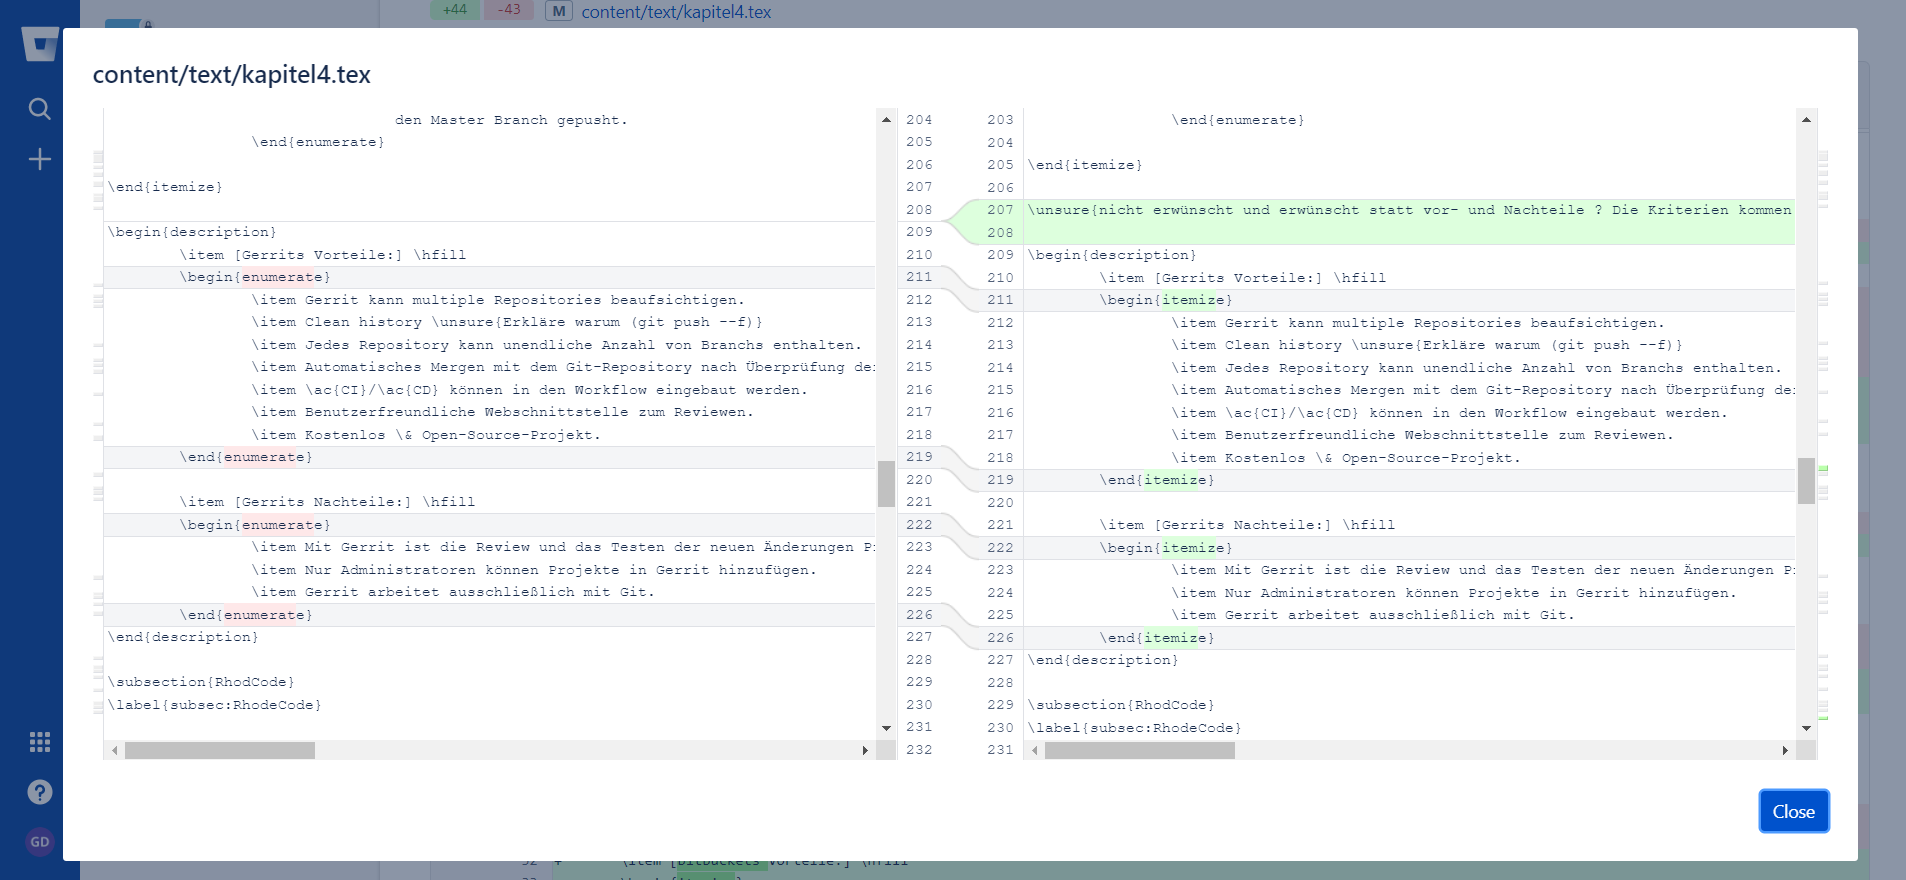
\includegraphics[width=1.0\textwidth]{Bitbucket side-by-side diffs}
	\caption[Bitbuckets Webanwendung side-by-side Änerungsvergleich]{Diffs side-by-side\\Eigenes Screenshot}
	\label{fig:Diffs_side-by-side}
\end{figure}

Im Gegensatz zu anderen Tools wird hier nur die Stelle, die geändert ist, markiert und nicht die ganze Zeile, die dazu gehört, was bei einer klaren Übersicht beiträgt.
Das Erstellen von Pull Request für den Feature Branch Übernimmt die Benutzer die an diesem Branch arbeiten. Beim Erstellen das Pull Requests wird das Feature Branch und das Ziel Branch ausgesucht und die Reviewer werden vom Autor ausgewählt. Die Beschreibung vom Pull Request wird die Nachrichten der Commits, die in dem Feature Branch eingecheckt wurden. Diese Beschreibung kann aber geändert werden.

Die Reviwer können das Pull Request auf Zeilen Ebene kommentieren, Todos erstellen (Allerdings nur nach dem Kommentar). Direkte Änderungen am Quelltext, die der Autor annehmen kann, sind nicht möglich (Mindestens mit der freien Version von Bitbucket-Cloud). Benutzer dieser Cloud-Version können keine Einschränkungen auf das Pull Request stellen, so kann der Feature Branch mit dem Ziel-Branch vom Autor zusammengeführt wird ohne ,dass die Reviewer das Pull Request zustimmen oder die von den Reviewern erstellte Todos gemacht zu haben.

\subsubsection{Self-Hosten}
\label{subsubsec:Bitbucket-self-host} 

Die Installation von Bitbucket-Server mit der Versionsnummer 7.2.3 erfolgte durch eine ZIP-Datei. Ein Verzeichnis für die Projekte und deren Repositories muss manuell erstellt werden und auf es in der Konfiguration-Datei \textit{set-bitbucket-home.sh} verwiesen werden, diese ist im Verzeichnis \textit{/atlassian-bitbucket-7.2.3/bin} zu finden. Wenn es kein Script für das Starten bzw. Stoppen von Bitbucket-Server erstellt wird, sind die ausführbare Dateien \textit{start-bitbucket.sh} und \textit{stop-bitbucket.sh} dafür verantwortlich.

Nachdem Starten von Bitbucket-Server können Projekte erstellt werden. In einem Projekt können neue Repositories angelegt oder auch von einem anderen Server geklont werden.
Bitbucket-Server hat im Vergleich zu der Cloud-Version mehr Funktionen wie beispielsweise das Abspalten von Branches oder der Änderungsvergleich zwischen ausgesuchten Commits, Versionen oder auch Branches. Die \cref{fig:Flexibilität des Änderungsvergleich} zeigt die Flexibilität des Änderungsvergleichs auf Bitbucket-Server.

\begin{figure}[H]
	\centering
	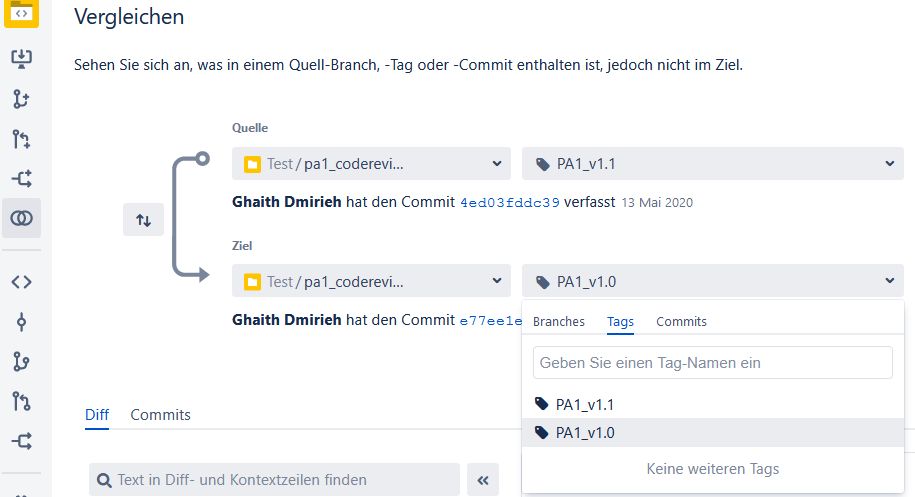
\includegraphics[width=1.0\textwidth]{BitbucketServerDiff}
	\caption[Flexibilität des Änderungsvergleichs auf Bitbucket-Server]{Flexibilität des Änderungsvergleichs \\Eigenes Screenshot}
	\label{fig:Flexibilität des Änderungsvergleich}
\end{figure}

Die Änderungen können sowohl inline als auch side-by-side angezeigt werden. Ein Beispiel dafür ist die \cref{fig:BitbucketServerSideBySide}

\begin{figure}[H]
	\centering
	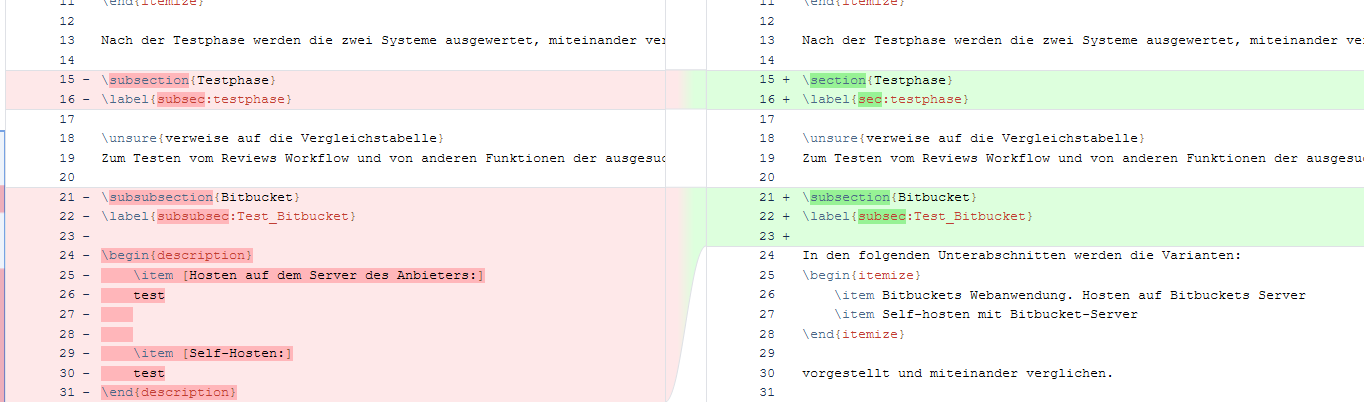
\includegraphics[width=1.0\textwidth]{BitbucketServerSideBySide}
	\caption[Side-by-side Änderungsvergleich auf Bitbucket-Server]{side-by-side Änderungsvergleich\\Eigenes Screenshot}
	\label{fig:BitbucketServerSideBySide}
\end{figure}

Weil ein Pull-Request auf Bitbucket nur zwischen Branches möglich ist, sollen Features in abgespaltene Branches entwickelt und mit einem Pull Request zum Review abgesendet werden. Beim Erstellen eines Pull Requests werden zwei Branches markiert \footnote{Der Feature Branch, wo die Änderungen/Features entwickelt wurden und der Ziel-Branch, mit dem der Feature Branch zusammengeführt werden soll}. Die Nachrichten von jedem Commit auf dem Feature Branch werden in der Beschreibung des Pull Requests auftauchen, die auch editiert werden kann. Es ist auch möglich Dateien mit dem Pull Request zu schicken.
Der letzte Schritt ist das Hinzufügen von Reviewer, die die Änderungen überprüfen, kommentieren und dann annehmen oder ablehnen können. Die \cref{fig:BitbucketServer Pull-Request} verdeutlicht die erwähnten Schritte.

\begin{figure}[H]
	\centering
	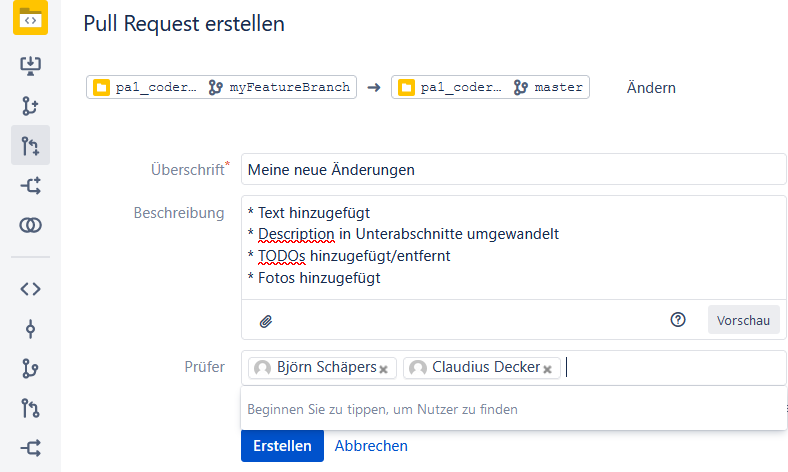
\includegraphics[width=1.0\textwidth]{BitbucketServer Pull-Request}
	\caption[Pull-Request auf Bitbucket-Server]{Pull-Request\\Eigenes Screenshot}
	\label{fig:BitbucketServer Pull-Request}
\end{figure}

Die Reviewer haben diverse Möglichkeiten, wie sie auf bestimmte Teile eines Pull Requests reagieren. Diese Möglichkeiten sind:
\begin{itemize}
	\item Kommentare, auf sie auch vom Autor wieder kommentiert werden kann. Beispiel \cref{fig:BitbucketServerKommentar}
	\begin{figure}[H]
		\centering
		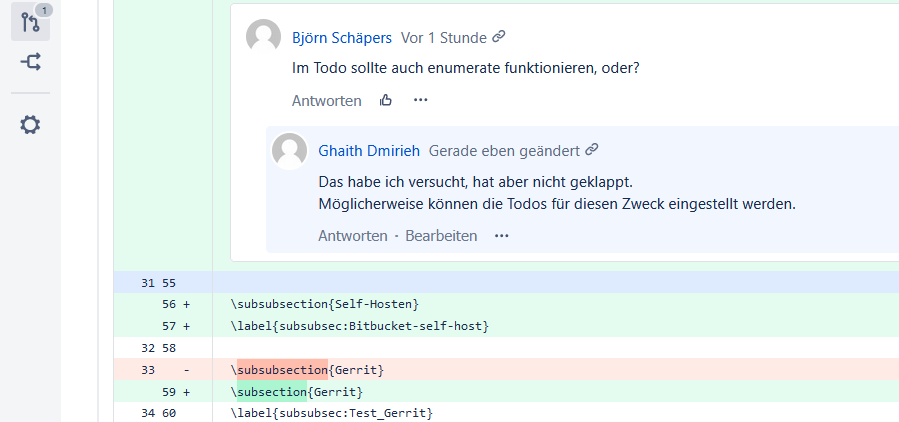
\includegraphics[width=1.0\textwidth]{BitbucketServerKommentar}
		\caption[Bitbucket-Server Kommentare]{Kommentare\\Eigenes Screenshot}
		\label{fig:BitbucketServerKommentar}
	\end{figure}
	
	\item Direkte Änderungen im Quelltext machen, die der Autor als Vorschläge bekommt. Bei der Annahme dieser Vorschläge muss der Autor eine commit Nachricht schreiben, da diese 				Annahme als ein neues commit gesehen wird. Beispiel \cref{fig:BitbucketServer Vorschläge}
	\begin{figure}[H]
		\centering
		\includegraphics[width=1.0\textwidth]{BitbucketServer Vorschläge}
		\caption[Bitbucket-Server Änderungsvorschläge]{Änderungsvorschläge\\Eigenes Screenshot}
		\label{fig:BitbucketServer Vorschläge}
	\end{figure}
	
	
	\item Erstellen von Task-Liste. Reviewer können Aufgaben/Todos stellen, die vom Autor nach dem Einchecken der Bearbeitung dieser Aufgaben als erledigt markiert werden können. Beispiel 	\cref{fig:BitbucketServer Tasklist}
	\begin{figure}[H]
		\centering
		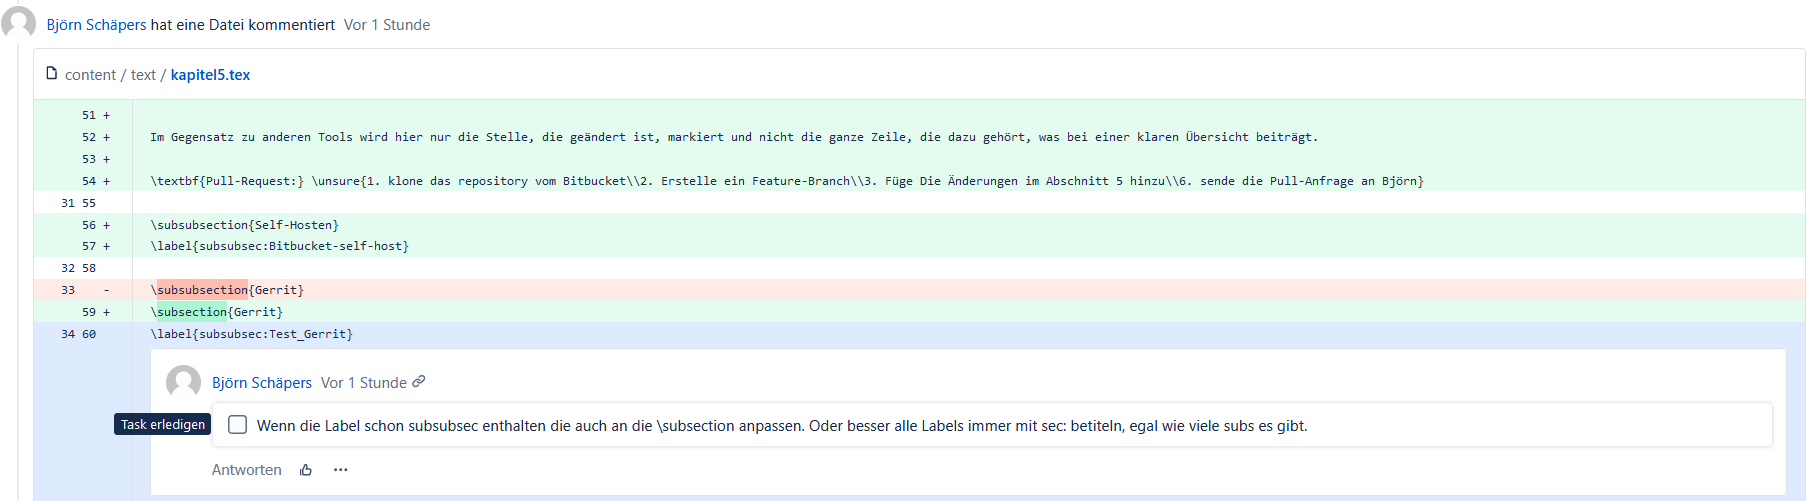
\includegraphics[width=1.0\textwidth]{BitbucketServer Tasklist}
		\caption[Bitbucket-Server Todos]{Todos/Aufgaben\\Eigenes Screenshot}
		\label{fig:BitbucketServer Tasklist}
	\end{figure}
\end{itemize}

Bitbucket-Server bietet die volle Kontrolle auf das Pul Request, sodass das Team den Workflow der Arbeit an seine Bedürfnisse anpassen kann. Ein Pull Request von einem Feature Branch kann beispielsweise nur dann mit dem Ziel-Branch zusammengeführt werden, wenn alle Reviewer oder gewählte Reviewer das Pull Request bestätigen. Eine andere Möglichkeit wäre es, dass keine offenen Aufgaben dabei sind, wenn es gemergt werden soll. Diese Einstellung sind auf \cref{fig:BitbucketServer Merge-Checks} zu sehen.
\begin{figure}[H]
	\centering
	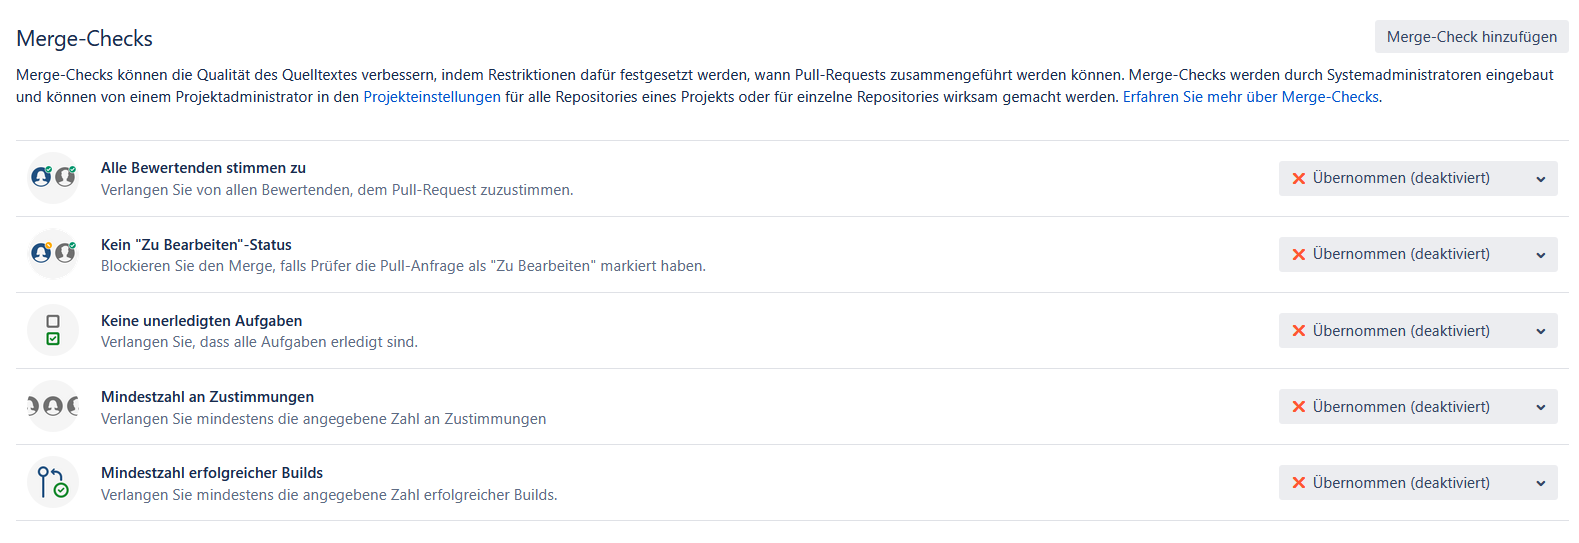
\includegraphics[width=1.0\textwidth]{Merge-Checks}
	\caption[BitbucketServer Merge-Checks]{BitbucketServer Merge-Checks\\Eigenes Screenshot}
	\label{fig:BitbucketServer Merge-Checks}
\end{figure}

Außerdem kann der Administrator eines Projekts Beschränkungen auf die Commits einrichten z.B., dass nur bestimmte Benutzer in einem Repository ihre Änderungen einchecken können. Die \cref{fig:BitbucketServer Commits-Kontrolle} zeigt die mögliche Beschränkungen.

\begin{figure}[H]
	\centering
	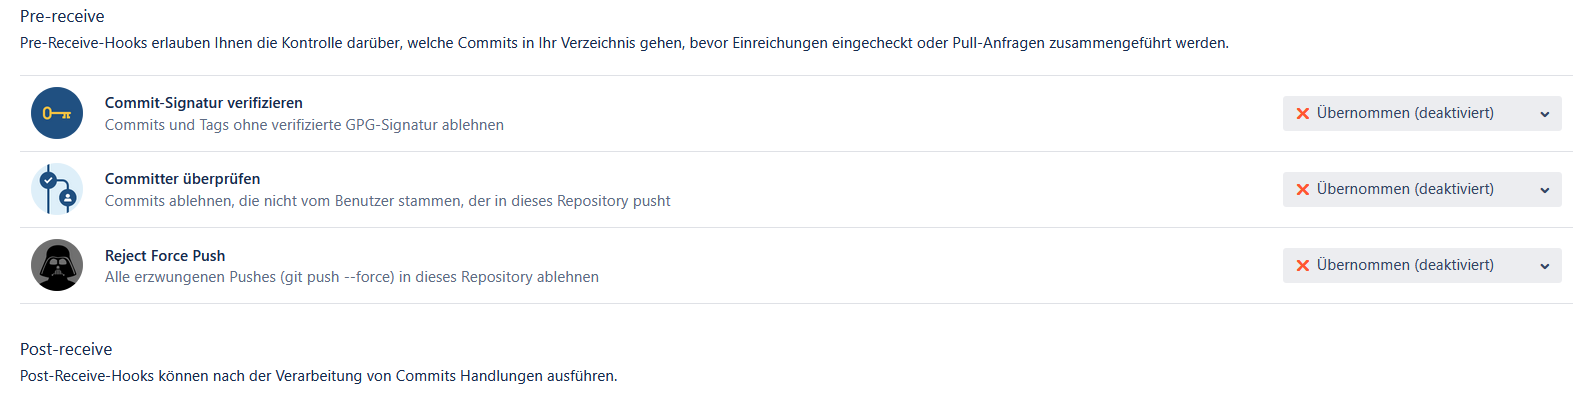
\includegraphics[width=1.0\textwidth]{Commits-Kontrolle}
	\caption[BitbucketServer Commits-Beschränkungen]{BitbucketServer Commits-Beschränkungen\\Eigenes Screenshot}
	\label{fig:BitbucketServer Commits-Kontrolle}
\end{figure}

Nach dem die Reviewer sich das Pull Request angeschaut,Kommentiert und Aufgaben sowie Vorschläge gestellt haben und der Autor diese bearbeitet hat, wurde das Feature Branch mit dem Ziel-Branch zusammengeführt.

\subsection{Gerrit}
\label{subsubsec:Test_Gerrit}

Gerrit unterscheidet sich von den anderen Quellcodeverwaltungssysteme, da Gerrit mehr Gewicht auf das Review legt. Das System arbeitet ausschließlich mit dem \ac{VCS} Git und hat keine Cloud Version. D.h. bei Gerrit handelt es sich nur um self hosten. Die Installation auf odin erfolgte durch ein \textit{.war} Datei, die mit dem Befehl

{\color{blue}
\begin{verbatim}
	java -jar gerrit.war init -d <Pfad zur .war Datei> 
\end{verbatim}}

\noindent initialisieren lässt. Nach der Initialisierung müssen noch wichtige Konfigurationen in der datei \textit{gerrit.config}, die im Verzeichnis \textit{gerrit-Verzeichnis/etc} zu finden sind, eingestellt werden. Wie beispielsweise die Authentifizierung oder auch, wo Gerrit seine Projekte und Repositories anlegt. Das Programm kann danach mit dem Befehl

{\color{blue} 
\begin{verbatim}
	gerrit.sh start
\end{verbatim}}

\noindent gestartet werden. Diese Datei befindet sich im Verzeichnis \textit{Gerrit-Verzeichnis/bin}. Gerrit ist ab jetzt lauffähig und Projekte können erstellt werden. Um ein Projekt zu erstellen gibt es verschiedene Methoden. Hier wird ein Projekt via SSH erstellt, was durch den Befehl

{\color{blue}
\begin{verbatim}
	ssh -p <port> <host> gerrit create-project <Name des Projekts>
\end{verbatim}}

\noindent erfolgen lässt. Gerrit kann einfach als ein neues Remote für ein bestehendes Repository hinzugefügt werden. Schließlich werden die Commits dieses Repositorys mit dem Befehl

{\color{blue}
\begin{verbatim}
	git push <remote name> <host>/<project name>
\end{verbatim}}

\noindent auf Gerrit hochgeladen.

\subsubsection{Reviews Workflow}
\label{subsubsec:Reviews Workflow bei Gerrit}

Der erster Schritt ist das Hinzufügen ein \textbf{Change-Id} für die Commits. Dieses ID erlaubt Gerrit, verschiedene Versionen derselben Änderungen, die überprüft werden sollen, miteinander zu verknüpfen. Dieser Schritt ist durch die zwei Befehle

{\color{blue}
\begin{verbatim}
	scp -p -P <port> <host>:hooks/commit-msg <Pfad zum Repository>/.git/hooks/
	chmod u+x .git/hooks/commit-msg
\end{verbatim}}

\noindent zu erreichen. Ab jetzt können Änderungen reviewt werden, indem man die Änderungen in den Branch \textit{HEAD:refs/for/master} von gerrit pusht. Beispiel für die Review-Webseite auf Gerrit stellt die \cref{fig:Gerrit-Review} vor.

\begin{figure}[H]
	\centering
	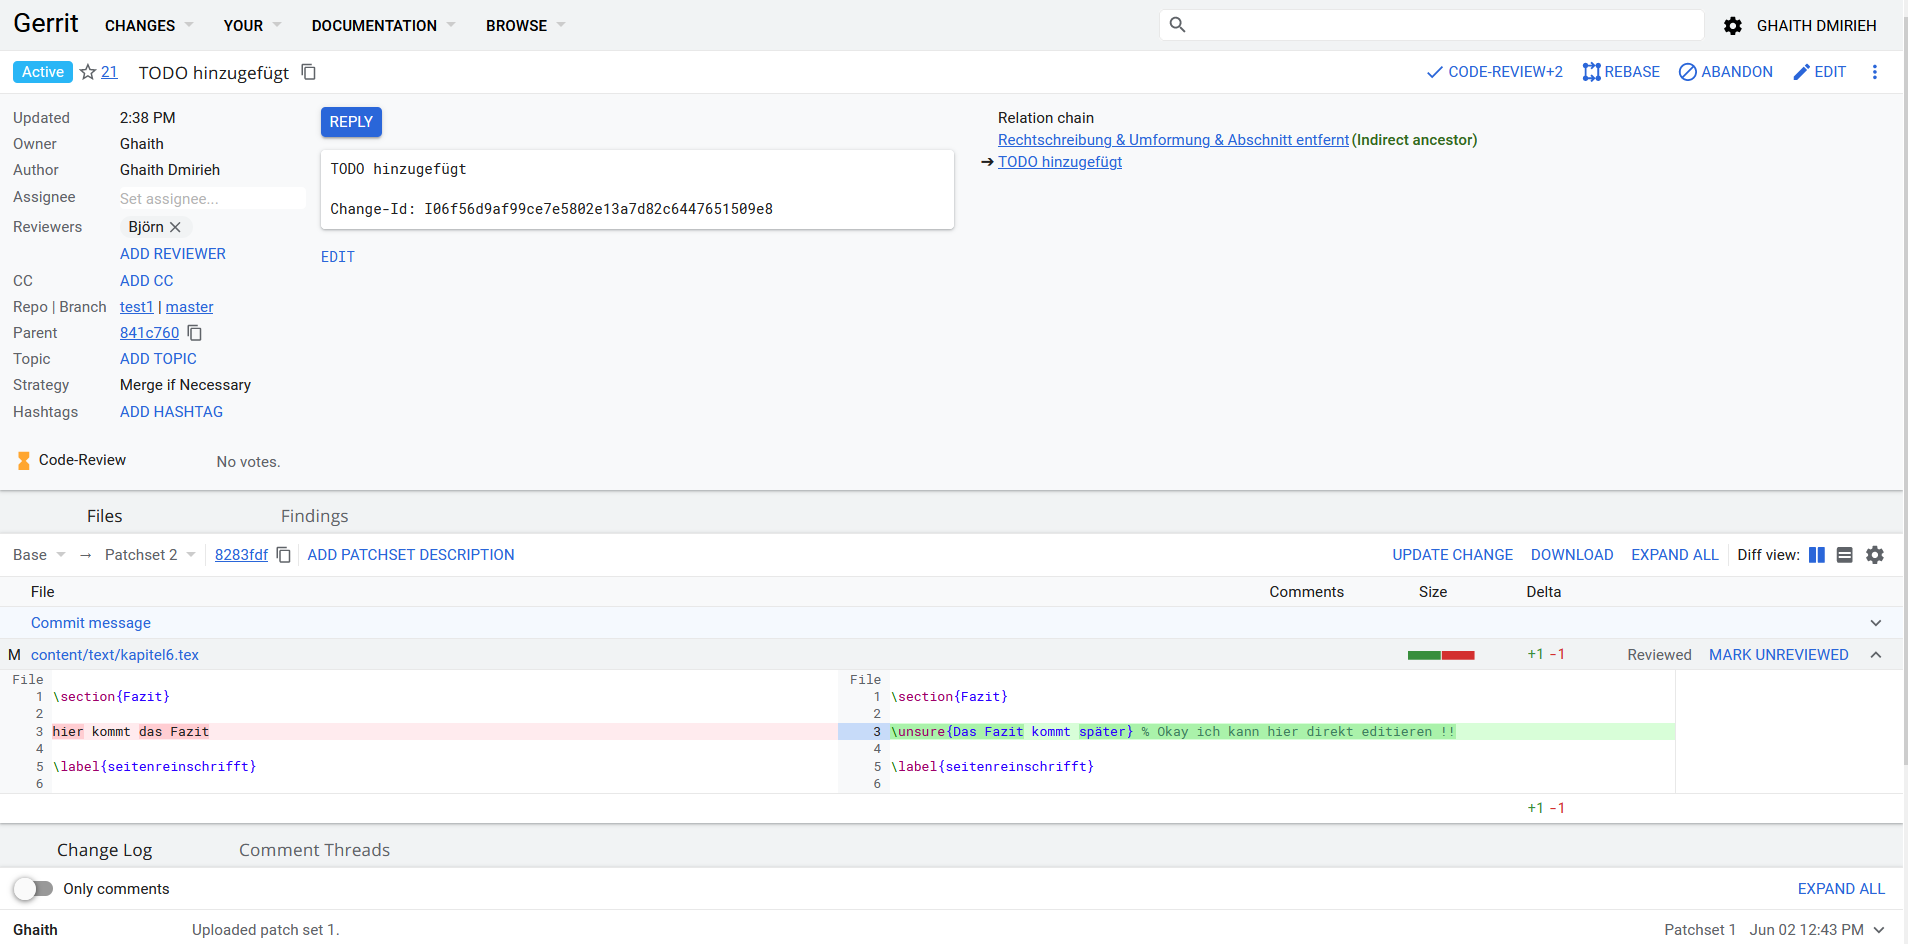
\includegraphics[width=1.0\textwidth]{Gerrit-Review}
	\caption[Gerrit Reviews Oberfläche]{Gerrit-Reviews Oberfläche\\Eigenes Screenshot}
	\label{fig:Gerrit-Review}
\end{figure}

Auf dieser Webseite können die Reviewer hinzugefügt werden, die eine E-Mail bekommen, dass sie zum Review eingeladen sind. Gerrit verschickt auch E-Mails an den Autor Änderungen oder Kommentare vom Reviewer. Ebenfalls bekommen wieder die Reviewer E-Mails, wenn der Autor auf ihre Kommentare reagiert.

Reviewer haben die Möglichkeit auf Zeilenebene die Änderungen zu kommentieren. Beispiel dafür zeigt die \cref{fig:Gerrit Reviewer-Kommentare} 

\begin{figure}[H]
	\centering
	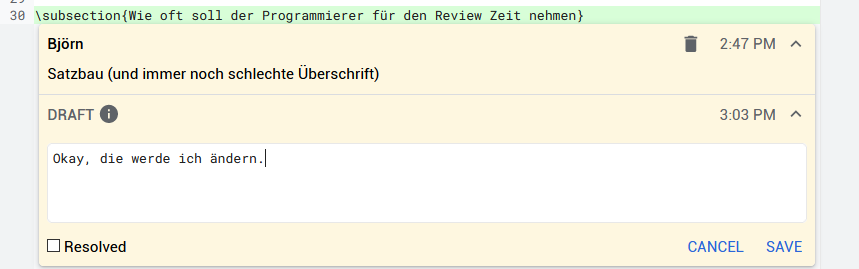
\includegraphics[width=1.0\textwidth]{Gerrit-Kommentar}
	\caption[Gerrit Reviewer-Kommentare]{Gerrit Reviewer-Kommentare\\Eigenes Screenshot}
	\label{fig:Gerrit Reviewer-Kommentare}
\end{figure}

Was auch Gerrit ermöglicht, sind die direkte Änderungen am Quelltext. Reviewer sind imstande, ihre Meinung direkt am Quelltext zu äußern. Der Autor kann dann mithilfe von Git diese Vorschläge von den Reviewern übernehmen. Der Prozess erfolgt durch das Edit-Modus in der Webseite von Gerrit. Die \cref{fig:Gerrit Edit-Modus} zeigt dieses Modus.

\begin{figure}[H]
	\centering
	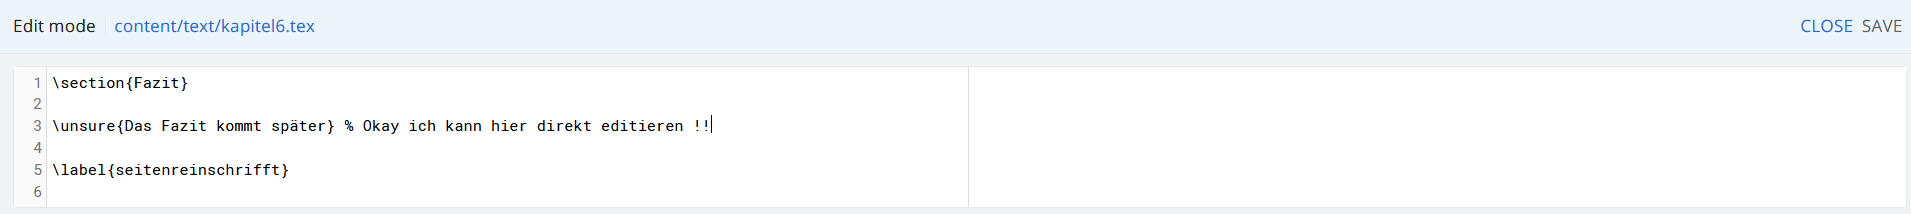
\includegraphics[width=1.0\textwidth]{Gerrit Edit}
	\caption[Gerrit Edit-Modus]{Gerrit Edit-Modus\\Eigenes Screenshot}
	\label{fig:Gerrit Edit-Modus}
\end{figure}

Selber auf die Nachricht des Commits Können die Reviewer kommentieren. Beispiel dafür ist die \cref{fig:Gerrit Kommentar auf Commits Nachricht}

\begin{figure}[H]
	\centering
	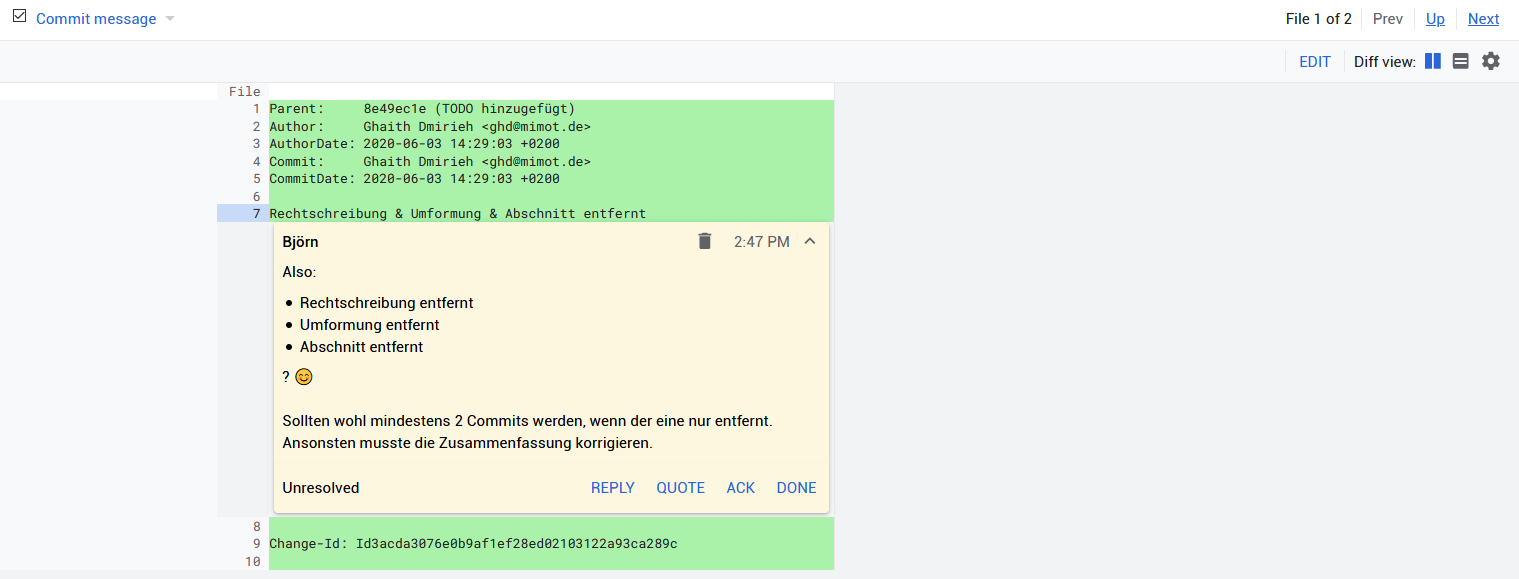
\includegraphics[width=1.0\textwidth]{Gerrit Kommentar auf Commits Nachricht}
	\caption[Gerrit Kommentar auf die Nachricht des Commits]{Gerrit Kommentar auf die Nachricht des Commits\\Eigenes Screenshot}
	\label{fig:Gerrit Kommentar auf Commits Nachricht}
\end{figure}

Nachdem die Reviewer die Änderungen anschauen und darauf reagieren und ihre Vorschläge machen, bekommen die Antworten vom Autor, diese sind Kommentare oder Bearbeitung der Änderungen. Falls die Reviewer die bearbeitete Änderungen gut finden, können sie diese bestätigen. Erst wenn die Änderungen bestätigt sind, kann das Commit mit dem Ziel-Branch zusammengeführt werden.

Die Reviewer können auf 5 Ebenen die Änderungen bewerten, diese sind
\begin{compactitem}
	\item \textbf{-2} Abgelehnt, Die Änderungen dürfen nicht gemergt werden.
	\item \textbf{-1} Ich bestätige sie nicht. Die Änderungen müssen bearbeitet werden.
	\item \textbf{0}  Keine Punktzahl
	\item \textbf{+1} Sieht für mich gut aus, aber jemand anderes muss sie noch bestätigen.
	\item \textbf{+2} Sieht gut aus. Ich bestätige sie.
\end{compactitem}

\subsection{Vergleich}
\label{subsec:Vergleich_Bitbucket_Gerrit}

Die zwei Systeme unterscheiden sich in zahlreichen Punkten, jedoch werden hier nicht alle in der Vergleichstabelle erscheinen, sondern nur die für die Abteilung wichtig sind. Diese Punkte verdeutlicht die \cref{table:Vergleichstabelle Gerrit & Bitbucket}

\begin{table}[h]
	\caption[Vergleichstabelle der ausgesuchten Systeme]{Vergleich der ausgesuchten Systeme}
	\centering
	\begin{tabular}{|c||c|c|}
			\hline 
			Eigenschaft & \textbf{Gerrit} & \textbf{Bitbucket Server} \\ 
			\hline 
			\textbf{\color{blue}{Review Workflow}} & Gerrit Branch & Pull Request \\ 
			\hline 
			\textbf{\color{blue}{Inline Diffs}} & \color{green}{\ja} & \color{green}{\ja} \\ 
			\hline 
			\textbf{\color{blue}{side by side Diffs}} & \color{green}{\ja} & \color{green}{\ja} \\ 
			\hline 
			\textbf{\color{blue}{Zugriffskontrolle auf Repo.}} & \color{green}{\ja} & \color{green}{\ja} \\ 
			\hline 
			\textbf{\color{blue}{Zugriffskontrolle auf den Reviews}} & \color{green}{\ja} & \color{green}{\ja} \\ 
			\hline 
			\textbf{\color{blue}{Vorschläge annehmen}} & \color{green}{\ja} & \color{green}{\ja} \\ 
			\hline 
			\textbf{\color{blue}{Patchsets}} & \color{green}{\ja} & \color{red}{\nein} \\ 
			\hline 
			\textbf{\color{blue}{E-Mail Benachrichtigungen}} & \color{green}{\ja} & \color{green}{\ja} \\ 
			\hline 
			\textbf{\color{blue}{Task-Liste}} & \color{red}{\nein} & \color{green}{\ja} \\
			\hline 
			\textbf{\color{blue}{Direkt Forken}} & \color{red}{\nein} & \color{green}{\ja} \\
			\hline 
			\textbf{\color{blue}{Diffs zwischen Commits/Tags/Branchs}} & \color{red}{\nein} & \color{green}{\ja} \\
			\hline 
			\textbf{\color{blue}{Kosten}} & Kostenfrei & Einmalige Zahlung \\
			\hline 
	\end{tabular} 
	\label{table:Vergleichstabelle Gerrit & Bitbucket}
\end{table}

\subsection{Auswertung}
\label{subsec:Auswertung}

Ganz wichtig zu erwähnen, dass um ein Pull Request zu erstellen, sollen die vom Pull Request betroffene Änderungen bereits in einem abgespaltenen Branch auf dem Remote-Repository stehen. D.h. Pull Requests sind mit Branchs engverbunden, was bestimmte Workflows erzwingt, demzufolge verringert dieser Prozess die Flexibilität vom \ac{VCS} Git, das die Entwickler ermöglicht, den Workflow an die Bedürfnisse des Teams anzupassen. Außerdem sind beispielsweise kleine Änderungen wie einen Fehler der korrigiert werden muss und seine Korrektur aus einer Zeile besteht, die jemanden anderen zuerst anschauen soll, nicht mehr flexibel, da dafür brauchen die Entwickler bei Bitbucket ein Branch zu erstellen. Im Gegensatz zu Gerrit kann man direkt im Haupt-Branch was ändern und ein Review dafür starten.

Bitbucket erleichtert die Arbeit mit seinen Funktionen in seiner Webseite, da man imstande ist, Branchs direkt in der Webseite zu erstellen oder sie abzuspalten. Im Gegensatz dazu hat Gerrit diese Funktionen nicht, da bei Gerrit es hauptsächlich um das Review geht. Beide Systeme können Zugriffsregeln auf die Repositories, Branchs oder auch wer reviewen darf erstellen, so dass nur bestimmte Entwickler daran arbeiten können.

Die Abteilung hat sich aus den folgenden Gründen

\begin{itemize}
	\item Bei Gerrit kann das Review unabhängig von dem Branch, an dem der Entwickler arbeitet, gestartet werden
	\item Ist der Entwickler mit seinen Änderungen fertig und will sie in das Haupt-Branch einchecken und inzwischen hat jemand an das Haupt-Branch was geändert, dann kann Gerrit 		mit damit umgehen
	\item Gerrit ist völlig kostenlos
\end{itemize}

für Gerrit entschieden.